\documentclass[utf8]{beamer}
\mode<presentation>
\usepackage[spanish]{babel}
\usepackage{multicol}
\useoutertheme{infolines} 
\usepackage{graphicx}
\usetheme{boxes}

\definecolor{lightblue}{rgb}{0,.5,1}
%\beamertemplateshadingbackground{lightblue!50}{lightblue!50}
%\setbeamercovered{transparent}


\begin{document}
\usebackgroundtemplate{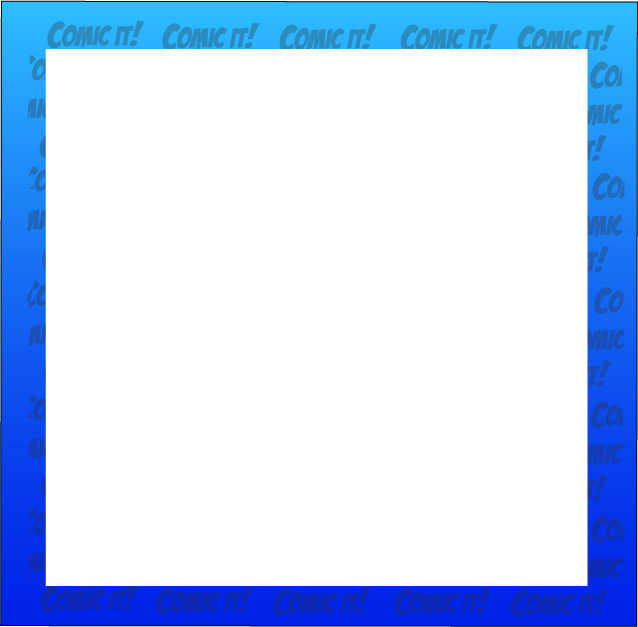
\includegraphics[width= \paperwidth, height=\paperheight]{imagenes/fondoazul.jpg}}
	\begin{frame}	
		\color{red}\textbf{\begin{center}{\Huge{¡Creando Historietas!}}\end{center}}				
		\pause
		\begin{center} 
				 
\includegraphics[width=0.5\textwidth]{imagenes/comicit.jpg} %Midifico el width para cambiar el tamaño%
		\end{center}
	\end{frame}
\usebackgroundtemplate{
\includegraphics[width= \paperwidth, height=\paperheight]{imagenes/fondoaz.jpg}}
	\begin{frame}	 	
		\color{red}\textbf{\begin{center}{\Huge{Autores}}\end{center}}
		\color{black}
		\begin{center}\huge{ 
			\pause
			- Ana Arias\\
			\pause
			- Liliana Ramos\\
			\pause
			- Denny Schuldt
			
			\pause
		}
			\normalsize
			\vspace{9mm}
			 Lenguajes de Programación
			\\2012 - II Término			
		\end{center}				
	\end{frame}




\begin{frame}	 	
		\color{red}\textbf{\begin{center}{\Huge{¡Comiquenado!}}\end{center}}
		\color{black}
		\begin{center}\huge{ 
			\pause
			- Ana Arias\\
			\pause
			- Liliana Ramos\\
			\pause
			- Denny Schuldt
			
			\pause
		}
			\normalsize
			\vspace{9mm}
			 Lenguajes de Programación
			\\2012 - II Término			
		\end{center}				
	\end{frame}

































\end{document}